%2multibyte Version: 5.50.0.2960 CodePage: 65001
%\input{tcilatex}
%\usepackage[latin1]{inputenc}
%\input{tcilatex}
%\input{tcilatex}
%\input{tcilatex}
%\\usepackage{harvard}
%\input{tcilatex}


\documentclass[harvard,11pt]{article}
%%%%%%%%%%%%%%%%%%%%%%%%%%%%%%%%%%%%%%%%%%%%%%%%%%%%%%%%%%%%%%%%%%%%%%%%%%%%%%%%%%%%%%%%%%%%%%%%%%%%%%%%%%%%%%%%%%%%%%%%%%%%%%%%%%%%%%%%%%%%%%%%%%%%%%%%%%%%%%%%%%%%%%%%%%%%%%%%%%%%%%%%%%%%%%%%%%%%%%%%%%%%%%%%%%%%%%%%%%%%%%%%%%%%%%%%%%%%%%%%%%%%%%%%%%%%
\usepackage{amssymb}
\usepackage{longtable}
\usepackage{amsfonts}
\usepackage{amsmath}
\usepackage{adjustbox}
\usepackage{placeins}
\usepackage{amsmath}
\usepackage[abs]{overpic}
\usepackage{linegoal}
\usepackage[FIGBOTCAP]{subfigure}
\usepackage{bbm}
\usepackage{bm}
\usepackage{booktabs}
\usepackage[round]{natbib}
\usepackage{tikz}
\usetikzlibrary{chains}
\usepackage{lipsum}
\usepackage{amsmath}
\usepackage{caption}
\usepackage{tabu}
\usepackage{amsmath}
\usepackage{physics}
\usepackage{booktabs}
\usepackage{graphicx,epstopdf}
\usepackage{setspace,caption}
\captionsetup{font=doublespacing}%
\usepackage{amsmath}
\usepackage[margin=1in]{geometry}
\usepackage{subfigure}
\usepackage{xargs}


\setcounter{MaxMatrixCols}{10}
%TCIDATA{OutputFilter=LATEX.DLL}
%TCIDATA{Version=5.50.0.2960}
%TCIDATA{Codepage=65001}
%TCIDATA{<META NAME="SaveForMode" CONTENT="1">}
%TCIDATA{BibliographyScheme=BibTeX}
%TCIDATA{LastRevised=Saturday, July 16, 2016 00:41:23}
%TCIDATA{<META NAME="GraphicsSave" CONTENT="32">}
%TCIDATA{Language=American English}

\newcommand*{\rom}[1]{\expandafter\@slowromancap\romannumeral #1@}
\newcommand{\R}{\mathbb{R}}
\newcommand{\E}{\mathbb{E}}
\newcommand{\N}{\mathbb{N}}
\newcommand{\I}{\mathbb{I}}
\newcommand{\Z}{\mathbb{Z}}
\newtheorem{theorem}{Theorem}
\newtheorem{acknowledgement}[theorem]{Acknowledgement}
\newtheorem{algorithm}[theorem]{Algorithm}
\newtheorem{axiom}[theorem]{Axiom}
\newtheorem{case}[theorem]{Case}
\newtheorem{claim}[theorem]{Claim}
\newtheorem{conclusion}[theorem]{Conclusion}
\newtheorem{condition}[theorem]{Condition}
\newtheorem{conjecture}[theorem]{Conjecture}
\newtheorem{corollary}{Corollary}
\newtheorem{criterion}{Criterion}
\newtheorem{definition}{Definition}
\newtheorem{example}{Example}
\newtheorem{exercise}[theorem]{Exercise}
\newtheorem{lemma}{Lemma}
\newtheorem{notation}[theorem]{Notation}
\newtheorem{problem}[theorem]{Problem}
\newtheorem{proposition}{Proposition}
\newtheorem{remark}{Remark}
\newtheorem{solution}{Solution}
\newtheorem{summary}[theorem]{Summary}
\newenvironment{proof}[1][Proof]{\textbf{#1.} }{\  \rule{0.5em}{0.5em}}
\newcommand{\cqfd}
{\mbox{}\nolinebreak \hfill \rule{2.5mm}{2.5mm}\medbreak \par}
\renewcommand{\cite}{\citeasnoun}
\geometry{left=0.8in,right=0.8in,top=0.8in,bottom=0.8in}
\renewcommand{\baselinestretch}{1.5}
%\input{tcilatex}
\begin{document}

\title{{Non-parametric estimation and inference for conditional mass based Granger causality measures for high-dimensional Markov chains with unknown transition matrices}}
\author{Xiaoxiao Ma\thanks{%
Institute for Transport Studies (ITS), University of Leeds. Address and email:
Institute for Transport Studies (ITS), University of Leeds, 34-40 University Road, Leeds, LS2 9JT}\\
%EndAName
University of Leeds\and Kaveh Salehzadeh Nobari\thanks{%
Department of Economics and Finance, Durham University. Address and email:
Department of Economics and Finance, Durham University Business School, Mill
Hill Lane, Durham, DH1 3LB.}\\
%EndAName
Durham University}
\date{\today \\
\textbf{This is a preliminary draft. Please do not cite or distribute without the permission of the authors.}}
\maketitle

%\renewcommand{\cite}{\citeasnoun} \renewcommand{\baselinestretch}{1.5}
\setlength{\baselineskip}{18pt}\pagestyle{plain}\newpage

\begin{center}
$\left. {}\right. ${\LARGE Non-parametric estimation and inference for conditional mass based Granger causality measures for high-dimensional Markov chains with unknown transition matrices}%
\begin{equation*}
\end{equation*}

\textbf{ABSTRACT}
\end{center}

\noindent \lipsum[2-3]

$\left. {}\right.$

\noindent \textbf{Journal of Economic Classification: C12, C13, C14%
}

$\left. {}\right. $

\noindent \textbf{Keywords}: Causality measures; Non-parametric estimation; Vine decomposition; Markov chains; Bernstein copula density; Local bootstrap.\newpage

%TCIMACRO{\TeXButton{\tableofcontents}{\tableofcontents}}%
%BeginExpansion
\tableofcontents%
%EndExpansion
\newpage

\section{Introduction \label{Introduction}}

\section{Motivation \label{Motivation}}
Consider the simple case of a first-order stationary two-state Markov chain, such as the one depicted below

\begin{center}
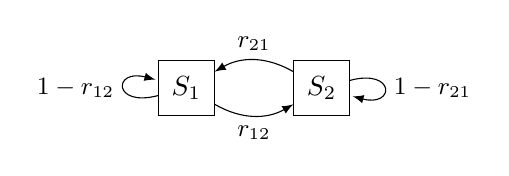
\begin{tikzpicture}[
mynode/.style={
  draw,
  minimum size=2em
  },
every loop/.append style={-latex},  
start chain=going right  
]
\foreach \Value in {1,2}
  \node[mynode,on chain] (s\Value) {$S_{\Value}$};
\path[-latex]
(s1) edge[bend right] node[auto,swap,font=\small] {$r_{12}$} (s2)
(s2) edge[bend right] node[auto,swap,font=\small] {$r_{21}$} (s1)
(s1) edge[loop left] node[left,font=\small] {$1-r_{12}$} (s1)
(s2) edge[loop right] node[right,font=\small] {$1-r_{21}$} (s2);
\end{tikzpicture}
\end{center}
with an \textit{unknown} transition matrix 
\[
\mathbf{P}=
\begin{bmatrix}
1-r_{12}&r_{12}\\
r_{21}&1-r_{21}
\end{bmatrix}
\]
where
\begin{equation}\label{eq: transition prob}
r_{ij}=P[X_t=i \mid X_{t-1}=j],\quad i,j\in\{1,2\}
\end{equation}
To estimate the conditional probabilties $r_{ij}$, we may express (\ref{eq: transition prob}) as follows
\begin{equation}
r_{ij}=\frac{P[X_t=i, X_{t-1}=j]}{P[X_{t-1}=j]}
\end{equation}
Furthermore, we know from the Theorem of \citet{sklar1959fonctions} that for the continuous variables $\{(X,Y,Z)\in\R\times\R\times\R\equiv \R^3\}$, the joint distribution function $F_{XYZ}(x,y,z)$ can be expressed using the marginal distributions and a copula function capturing the depedence, - i.e. 
\begin{equation}\label{eq: copula}
F(x,y,z)=C(F_X(x),F_Y(y),F_Z(z))
\end{equation}
where $F_{\kappa}(.)$ for $\kappa=X, Y, Z$ is the marginal distribution function of variable $\kappa$ and $C(F_X(.),F_Y(.),F_Z(.))$ is a copula function on $[0.1]^3$ that captures the dependence of $(X,Y,Z)$. If we take the derivative of $\ref{eq: copula}$ with respect to $(x,y,z)$, we obtain the joint density funciton of $(X,Y,Z)$:
\begin{equation}\label{eq: density}
f(x,y,z)=f_X(x)\times f_Y(y)\times f_Z(z)\times c(F_X(x),F_Y(y),F_Z(z))
\end{equation}
\section{Copula-based Granger causality measures for qualitative processes \label{Copula-based Granger causality measures for qualitative processes}}

Consider a homogeneous Markov process of order one with a state-space consisting of finite elements and the transition matrix
\begin{equation}\label{eq: transition matrix}
P[X_t=i,Y_t=k\mid X_{t-1}=j,Y_{t-1}=l]=p_{i,k\mid j,l},
\end{equation}
for $i,j=1,\cdots,J$ and $k,l=1,\cdots,L$. Furthermore, the invariant initial probability is given by
\begin{equation}
P[X_t=i,Y_t=k]=\pi_{i,k}
\end{equation}
with $i=1,\cdots,J$ and $k=1,\cdots,L$. \citet{gourieroux1987kullback} show that the causality measure from $X$ to $Y$ is defined by
\begin{equation}\label{eq: 1989measure}
C(X\rightarrow Y)=\sum\limits_{j=1}^{J}\sum\limits_{l=1}^{L}\pi_{j,l}\left\{\sum\limits_{k=1}^{L}p_{k\mid j,l}\log\frac{p_{k\mid j,l}}{p^y_{k\mid l}}\right\}
\end{equation}
where
\[
p_{k\mid j,l}=\sum_{i=1}^{J}p_{i,j\mid k,l}=P[X_t=i\mid X_{t-1}=j,Y_{t-1}=l]\quad\text{and}\quad p^{y}_{k\mid l}=\frac{\sum\limits_{k=1}^L\sum\limits_{l=1}^Lp_{i,k\mid j,l}\pi_{j,l}}{\sum\limits_{l=1}^L\pi_{j,l}}
\]
However, expression (\ref{eq: 1989measure}) is difficult to evaluate. 

\[
P[X_t=i,Y_t=k\mid X_{t-1}=j,Y_{t-1}=l]=p_{i,k\mid j,l}
\]
\[
f[x_t^*,y_t^*\mid x_{t-1}^*,y_{t-1}^*]=p_{i,k\mid j,l}
\]
with
\[
X_t^*=X_t+U-1,\quad U\sim Uniform[0,1]
\]
\begin{eqnarray*}
f[x_t^*,y_t^*, x_{t-1}^*,y_{t-1}^*]/f(x_{t-1}^*,y_{t-1}^*)=\\
f(x_t^*)f(y_t^*)f(x_{t-1}^*)f(y_{t-1}^*)c(F(x_t^*),F(y_t^*),F(x_{t-1}^*),F(y_{t-1}^*))/f(x_{t-1}^*)f(y_{t-1}^*)c(F(x_{t-1}^*),F(y_{t-1}^*)
\end{eqnarray*}

\begin{eqnarray*}
f[y_t^*, x_{t-1}^*,y_{t-1}^*]=f(y_t^*)f(x_{t-1}^*)f(y_{t-1}^*)c(F(y_t^*),F(1),F(y_{t-1}^*),F(x_{t-1}))
\end{eqnarray*}


\section{Estimation and inference \label{Estimation and inference}}

\subsection{Estimation \label{Estimation}}

\subsection{Inference \label{Inference}}

\section{Measuring causality in high-dimensional Markov chains \label{Measuring causality in high-dimensional Markov chains}}
\section{Monte Carlo simulations \label{Monte Carlo simulations}}

\subsection{Bootstrap bias-corrected estimator of Granger causality measures \label{Bootstrap bias-corrected estimator of Granger causality measures}}

\subsubsection{Bootstrap bias-correction \label{Bootstrap bias-correction}}

\subsubsection{Simulation study \label{Simulation study}}

\subsection{Empirical size and power \label{Empirical size and power}}

\section{Empirical application\label{Empirical application}}


\section{Conclusion \label{Conclusion}}

\newpage
\bibliographystyle{apa}
\bibliography{References_Final}

\newpage

\section{Appendix: Proofs \label{Appendix: Proofs}}
\end{document}